\documentclass[12pt,letterpaper]{article}
\usepackage{times} 
%\renewcommand{\rmdefault}{ptm}
%\renewcommand{\sfdefault}{phv} % leaves tt as computermodern
\usepackage{graphicx}
\usepackage{html}
\usepackage[lmargin=1in,rmargin=1in,tmargin=1in,bmargin=1in,headsep=18pt,
  footskip=36pt, headheight=16pt]{geometry}
\usepackage{boxedminipage}
  \setlength\fboxsep{2mm}
%\usepackage{wrapfig}
%\usepackage{floatflt}
%\usepackage{setspace}
\usepackage{paralist}
  \setlength\plitemsep{2pt}
  \setlength\pltopsep{4pt}
\usepackage[round]{natbib} % for ecology
\usepackage{sectsty} 
  \sectionfont{\sffamily \bfseries \scshape \raggedright \large} 
  \subsectionfont{\sffamily \mdseries \itshape \normalsize
    \raggedright}
  \subsubsectionfont{\mdseries \itshape \normalsize}
%  \renewcommand \thesection{\roman{section}.}
\usepackage[small,bf]{caption2}
  \renewcommand{\captionlabeldelim}{}
  \captionstyle{flushleft}
  \onelinecaptionsfalse
%\usepackage{array}
\usepackage[usenames]{color}
  \definecolor{darkblue}{rgb}{0,0,0.3}
\hypersetup{latex2html, colorlinks=true,linkcolor=darkblue,urlcolor=darkblue,
  citecolor=darkblue}
%\usepackage[draft]{hyperref}
  \urlstyle{same}
\addtolength{\skip\footins}{3mm}
\addtolength{\footnotesep}{3mm}
\usepackage{tabularx}
%\usepackage{multirow}
%\usepackage{longtable}
\usepackage{fancyhdr}
%\usepackage{multicol} % \usepackage{multicol,ragged2e}
%  \addtolength\columnsep{4pt}
%\usepackage{lineno}
\usepackage{comment}
%\usepackage{svn}
%  \SVN $Revision: 252 $
%  \SVN $Date: 2011-08-25 06:04:51 +0700 (Thu, 25 Aug 2011) $
% Activated with svn propset svn:keywords "Date Revision" phylocom_manual.tex

%%%% Set version here:
\newcommand{\phylocomversion}{4.2} 


\begin{document}
\sloppy
\thispagestyle{empty}

\begin{center}
{\sffamily \bfseries \scshape {\huge P~h~y~l~o~c~o~m \\}}
\bigskip \bigskip
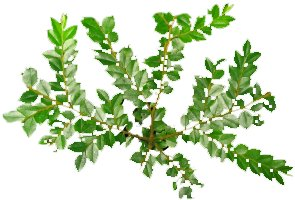
\includegraphics[width=5cm]{img/phylocom.jpg}
\bigskip \bigskip

{\sffamily \bfseries \scshape {\Large Software for the Analysis of \\
Phylogenetic Community Structure and \\ Character Evolution \\ (with
Phylomatic and Ecovolve)\\}

\bigskip \bigskip

{\Large User's Manual \\}
\bigskip \bigskip
{\sffamily \bfseries \scshape \large Version \phylocomversion\\}
\bigskip \bigskip

{\textnormal \copyright} 2011 Campbell Webb, David Ackerly, Steve Kembel
\bigskip \bigskip

{\large Cam Webb\\}
Arnold Arboretum of Harvard University\\
\htmladdnormallink{cwebb@oeb.harvard.edu}{mailto:cwebb@oeb.harvard.edu}\\

\bigskip \bigskip

{\large David Ackerly\\}
University of California, Berkeley\\
\htmladdnormallink{dackerly@berkeley.edu}{mailto:dackerly@berkeley.edu}

\bigskip \bigskip

{\large Steve Kembel\\}
University of Oregon\\
\htmladdnormallink{skembel@uoregon.edu}{mailto:skembel@uoregon.edu}
  }
\end{center}



\newpage

% -- FANCYHDR -----------------------------------------------------------
\pagestyle{fancy}
 % \lfoot{\footnotesize Revision \SVNRevision}
 % \rfoot{\footnotesize \SVNDate}
 \chead{} 
 \rhead{\scshape Phylocom Manual}
 \cfoot{\thepage} 
 \lhead{\em Webb, Ackerly and Kembel} 
 \renewcommand{\headrulewidth}{0.4pt} 
 \renewcommand{\footrulewidth}{0.4pt} 
% ---------------------------------------------------------------------------

\tableofcontents % comment out when using latex2html

\newpage

\section{Introduction}

{\scshape Phylocom} is a command-line application for manipulating
ecological and phylogenetic data, calculating various metrics of
phylogenetic and phenotypic community structure, and measuring trait
conservatism and trait correlations.

We have developed a system to help take the evolutionary ecologist
easily through the steps needed in an analysis of phylogenetic
community structure or trait evolution. {\scshape Phylomatic} can be used
to rapidly develop a phylogeny for any plant community.  This
phylogeny can then be input into the {\scshape phylocom} program to measure
phylogenetic relatedness among species occurring together in samples,
test hypotheses of community structure, or quantify patterns of trait
evolution. If estimates exist for the ages of any node, these can be
incorporated, as can branch lengths from other sources. {\scshape Ecovolve}
is a phylogeny growth simulator, using the same file formats as the
other tools. These tools will remain command-line programs, so
that they can easily be used inside other programs and shell-scripts.

\subsection{New in Version 4.2}
\begin{itemize}
 \item Phylomatic no longer outputs a branch length for the root node;
   the presence of this BL (allowed by the Newick definition) was
   causing parsing errors in other applications.
\end{itemize}

\subsection{New in Version 4.1}
\begin{itemize}
 \item Renamed \verb|comdistnn| function to \verb|comdistnt| for
   consistency
 \item Added null model testing to \verb|comdist|/ \verb|comdistnt|
   functions
 \item Windows version now compiled with \htmladdnormallink{\sc
   mingw32}{http://www.mingw.org/}, rather than {\sc djgpp}.  This
   should help with some of the memory issues some Windows
   users were experiencing.  A \verb|phylocom.bat| file is also
   included to assist in opening a \verb|CMD.EXE| console window. 
\end{itemize}

\subsection{New in Version 4.0}

\begin{itemize}
 \item Added code to detect line endings (Mac/Windows/Unix) and adjust
   automatically.
 \item Added \verb|rao| function to calculate phylogenetic diversity.
 \item Updated  \verb|comstruct| and  \verb|comdist| to use -a switch
to incorporate abundance into phylogenetic distance calculations.  NB:
see \citet{hardy2008tes} for a discussion of important issues
concerning abundances and Type I and II errors in detection of significant
phylogenetic structure.
 \item  \verb|comtrait| function calculates trait dispersion within communities.
 \item Modified calculation of phylogenetic signal.
\end{itemize}

\section{Installation}

\subsection{Mac OS X}

Universal binaries for OS 10.5 are included in the \verb|mac|
directory. If these do not run (perhaps if you are using an older
version of OS X), you may want to build from scratch: acquire the OS X
Developer Tools Installer from the Apple website (you may have to
register as a developer), or from your installation discs, and
install.  Then follow the instructions below for a UNIX build.

This is {\bf command-line software}. You need to run it in a terminal
window (\verb|/Applications/|\-\verb|Utilities/|\-\verb|Terminal.app|).

To make {\scshape phylocom} available anywhere (i.e., not always
requiring the executable in the same directory as your data files),
create a \verb|bin/| directory under your home directory, and add this
line to your \verb|.bash_profile| file:
\begin{verbatim}
  PATH=$PATH:$HOME/bin:. ; export PATH
\end{verbatim}
or this line to your \verb|.tcshrc| file, if you are running the
\verb|tcsh| shell:
\begin{verbatim}
  set path=(. ~/bin $PATH)
\end{verbatim}

\subsection{Linux/Other Unix}

Rather than provideing precompiled binaries for each architecture,
unix users should compile locally.  These commands should work:
\begin{verbatim}
  $ cd Desktop          # or to wherever you save the zip file
  $ unzip phylocom.zip
  $ cd phylocom-X       # replace X with version no.
  $ cd src
  $ make
  $ ./phylocom
\end{verbatim}
If your system does not use \verb|gcc|, edit the \verb|Makefile| to
reflect your C-compiler.

% Make sure gcc and awk or gawk are installed.  Later, check the first
% line of the awk-scripts nex2fy and new2fy to make sure they point to
% the awk/gawk executable. Gawk is recommended since the scripts use
% some higher functions of awk, not available in all older awk versions.

To make {\scshape phylocom} available anywhere (i.e., not always
requiring the executable in the same directory as your data files),
create a \verb|bin/| directory under your home directory, and add this
line to your \verb|.bash_profile| file:
\begin{verbatim}
  PATH=$PATH:$HOME/bin:. ; export PATH
\end{verbatim}
or this line to your \verb|.tcshrc| file, if you are running the
\verb|tcsh| shell:
\begin{verbatim}
  set path=(. ~/bin $PATH)
\end{verbatim}

\subsection{Windows}

Windows 32-bit binaries are included in the \texttt{w32}
directory. These binaries were compiled with
\htmladdnormallink{\texttt mingw32}{http://www.mingw32.org/} under
Linux (see \verb|Makefile|).  The binaries run in the Windows console
(usually found at: \verb|c:\windows\system32\cmd.exe|); note that this
shell is no longer the same as {\sc ms-dos}, although most of the
commands behave as before (see
\htmladdnormallink{http://commandwindows.com/}{http://commandwindows.com/}
for an excellent introduction to the Windows console).

If you need to recompile in Windows, use
\htmladdnormallink{\texttt{mingw32}}{http://www.mingw.org/}, or you
can install and use the \verb|cygwin| tools.

\label{unixpath}In order to access {\scshape phylocom} from anywhere in your directory
tree, create a directory where you want \verb|phylocom.exe| to live
(e.g., \verb|C:\PHYLOCOM|).  Right click the My Computer icon, choose
Properties, then click on advanced system settings, then click on
environment variables. From there, add the name of the directory where
you have placed the {\scshape phylocom} executable to the end of the
list of directories in the path. Copy the executables (\verb|.exe|
files) to this new directory, open a new command prompt window, and
you should be able to type \verb|phylocom| and have the program run.
This is the same as adding these lines to a batch file:
\begin{verbatim}
  path = %PATH%;C:\phylocom
\end{verbatim}
 
This is {\bf command-line software}. You need to run it in a console
window.  You can acces the console via (one of):
\begin{compactenum}
  \item Start Menu $\to$ Applications $\to$ Accessories $\to$ Command
    prompt
  \item Start Menu $\to$ Run, and type \verb|CMD| 
  \item Double clicking on the \verb|phylocom.bat| file.  This must be
    in the same directory as the executables, unless you have set the
    path, as above.
\end{compactenum}

If you are frequently using a particular {\sc phylocom} function, you
can also make custom shortcuts (a tip from an anonymous reviewer):
\begin{compactenum}
  \item Place your executable \verb|phylocom.exe| in a standard
    location (e.g., \verb|"C:\PROGRAM FILES\PHYLOCOM\"|)
  \item Create a shortcut to \verb|phylocom.exe| and rename it (e.g.,
    \verb|phylocom_comstruct|).
  \item Opening the properties of
    the shortcut, and in the Target box, enter
    \verb|"C:\PROGRAM FILES\PHYLOCOM\PHYLOCOM.EXE" COMSTRUCT > OUT.TXT|
  \item Leave the `Run In' box blank
\end{compactenum}
The shortcut can now be copied and dropped into any directory where
you want to run an analysis (with data files named to the default
names).  Alternatively, you can put the following (all in one line) in
the `Target' box, to run the program in a console, which will stay
open after the program has run:
\begin{verbatim} 
  C:\WINDOWS\system32\cmd.exe /k 
  "c:\program files\phylocom\phylocom.exe" 
  comstruct > out.txt
\end{verbatim}

\section{Input file formats}

{\scshape Phylocom} uses plain text files as input (i.e., not propriety
binary formats such as \verb|.xls| and \verb|.doc|).  This facilitates
connecting the software as part of an analysis or simulation chain,
because text processing tools (e.g., \verb|sed|, \verb|awk|,
\verb|perl|) can be used to re-format files, etc.  However, because
one has access to the internals of the data files in this way, one
must be extra careful with accuracy of formatting: no extra spaces,
tabs, etc.  Learning to use a good text editor will greatly help; we
recommend
\htmladdnormallink{TextWrangler}{http://www.barebones.com/products/textwrangler/}
for Mac and
\htmladdnormallink{Notepad-plus}{http://notepad-plus.sourceforge.net/}
for Windows.

{\it Note}: As of version 4.0, {\scshape phylocom} recognizes the
line-endings (\textsc{unix}, Mac, Windows) used in each file.  This
should save a lot of wasted time!  However, your line-endings must be
consistent within each file.

\subsection{Tree preparation}

{\scshape phylocom} reads Newick-format phylogenies directly. See:
\begin{itemize}
\item[]
  \htmladdnormallink{http://evolution.genetics.washington.edu/phylip/newicktree.html}{http://evolution.genetics.washington.edu/phylip/newicktree.html},
  and
\item[]
  \htmladdnormallink{http://evolution.genetics.washington.edu/phylip/newick\_doc.html}{http://evolution.genetics.washington.edu/phylip/newick_doc.html}
\end{itemize}
for definitions of the Newick standard.  The default file name is
\verb|phylo|, but other phylogeny files can be specified using the
\verb|-f| filename option.  Plain Newick format phylogenies are also
used by {\scshape phylip}.

The basic Newick format used by {\scshape phylocom} is:
\begin{verbatim}
  ((A,B),C);
\end{verbatim}
The full complexity Newick format that can be read by {\scshape phylocom} is:
\begin{verbatim}
  ((A_sp:1.1,B2-sp:2.2)clade1:1.0[a comment],c_sp:0.5);
\end{verbatim}

Please note: 

\begin{itemize}
  \item Taxa and interior names must begin with \verb|A-Z| or
    \verb|a-z|, not a number,
  \item Branch lengths will be assumed to be 1.0 if not present,
  \item Comments are ignored,
  \item The root node should not have a branch length if other branch
    lengths are given,
  \item There should be no whitespace or line-endings within the tree,
  \item Trailing spaces/line-endings at the end of the phylo file are
    OK, but not in any other file format used by {\scshape phylocom},
  \item Multiple Newick strings (as in {\scshape phylip} \verb|intree|
    files) are currently not allowed in the \verb|phylo| file,
  \item The basal node must be a dichotomy, not a polytomy.
\end{itemize}

\subsubsection{Newick and {\scshape nexus}}

One of the standard file formats for phylogenies is {\scshape nexus}.  If
you open a {\scshape nexus} file with a text editor, you will see one or
more Newick strings in the TREES section.  You may be able to simply
cut out the Newick string and paste into a new \verb|phylo| file.
However, some programs write by default a translation of the taxon
names into numbers.  These translated Newick strings need to be
`un-translated' before using in {\scshape phylocom}.  A simple way to get a
Newick string out of a {\scshape nexus} file is to open the {\scshape nexus}
file in \htmladdnormallink{Mesquite}{http://mesquiteproject.org/},
open a tree window (Taxa\&Trees $\to$ New Tree Window) for the stored
tree (Stored Trees), click on the `Text' tab, and save the text page
to a file (File $\to$ Save Window as Text...).  In the saved file,
edit out everything but the Newick string.

\subsection{Sample preparation}
 
{\scshape phylocom} accepts various kinds of sample data. Samples may
represent subsets of the phylogenetic tree, or ecological data
matrices (measurements of species abundance or occurrence in samples
of some sort). The default file name is \verb|sample|, but other sample files
can be specified using the \verb|-s filename| option.

The sample file has the following format: 

\begin{itemize}
\item 3 columns, tab delimited, sorted by column 1
\item one row per taxon: 
\begin{enumerate}
\item Sample (plot, quadrat, trap,
etc.) name (character string, no spaces, should begin with \verb|[A-Za-z]|) 
\item Abundance (integer; leave as 1 for presence/absence data)
\item Species code (string, same as in \verb|phylo|, should begin with \verb|[A-Za-z]|) 
\end{enumerate}
\item all species in
this table MUST be included in \verb|phylo|
\end{itemize}
        
You can wrestle your data into this format pretty easily, using a
stats package or spreadsheet. Look at the included example file
\verb|sample| for an idea of what the file should look like.  The
current version has been tested to work with fairly large ecological
data sets as sample files (e.g., 400 species and 5,000 samples).

\subsection{Traits preparation}

Any number of characters can be included in the \verb|traits|
file. Note that missing trait values are not allowed, and the list of
taxa in \verb|traits| must exactly match the terminal taxa in the phylo
file. The default file name is \verb|traits|, but other trait files can be
specified using the \verb|-t filename| option.

The first line of traits must read:
\begin{verbatim}
  type<TAB>n<TAB>n<TAB>... [up to the number of traits]
\end{verbatim}
where \verb|n| indicates the type of trait in each of the four
columns:

\begin{itemize}
\item[\texttt{0}] for binary (only one binary trait may be included, and it must be in the first column)
\item[\texttt{1}] for unordered multistate (no algorithms currently implemented)
\item[\texttt{2}] for ordered multistate (currently treated as continuous)
\item[\texttt{3}] for continuous
\end{itemize}

Optional: The second line can start with the word \verb|name| (lower case
only) and then list the names of the traits in order. These will
appear in the full output file.

Subsequent lines should have the taxon name, which must be identical
to its appearance in \verb|phylo|, and the data columns separated by
tabs. See the example traits file distributed with the program.

\section{Using {\scshape phylocom}}
\label{s:usingphylocom}

NOTE: Investing in a basic guidebook for {\scshape unix} or {\scshape
  dos}/Windows console will be very worthwhile in the long run.
Alternatively, the web is full of useful pages, e.g., Google:
\htmladdnormallink{`introduction to
  unix'}{http://www.google.com/search?q=introduction+to+unix} or
\htmladdnormallink{`commandline
  Windows'}{http://www.google.com/search?q=commandline+Windows}.

Try this software first with the included example files.  Either i) copy these
files to the same directory as the executables, or ii) make the
executables universally findable on your system (see
\S~\ref{unixpath}), and just \verb|cd| to where your (demo or real)
input files are.  Then just type:
\begin{verbatim}
  $ phylocom
\end{verbatim}
(NOTE, the \verb|$| symbol in this manual indicates the {\it command
  prompt}; do not type this symbol, only what follows it).  If you are
using OS X/UNIX and haven't placed the {\scshape phylocom} executable
in your path (see \S~\ref{unixpath}), type:
\begin{verbatim}
  $ ./phylocom
\end{verbatim}
In Windows console, just double-click on the \verb|phylocom.bat| file,
or manually \verb|cd| to the correct directory, and type:
\begin{verbatim}
  C:\SOME\PATH>PHYLOCOM.EXE
\end{verbatim}
or just:
\begin{verbatim}
  C:\SOME\PATH>phylocom
\end{verbatim}
A welcome screen should appear. The format for the various options is:
\begin{verbatim}
  $ phylocom method [optional parameters]
\end{verbatim}
Basic information can be obtained at any time by calling: 
\begin{verbatim}
  $ phylocom help
\end{verbatim}

Output from the programs is written to the screen (generally
\verb|/dev/stdout|, although some warnings are sent to
\verb|/dev/stderr|).  In order to capture the output into a file, it
must be redirected to a filename, e.g.:
\begin{verbatim}
  $ phylocom comstruct > myoutput.txt
\end{verbatim}
or:
\begin{verbatim}
  $ phylocom bladj > mytree.new
\end{verbatim}
This syntax works on both {\scshape unix} systems and in the Windows console.

\section{Basic data extraction and manipulation}

A number of algorithms have been included to assist in summarizing
data and converting between formats.  These are generally simple to
write, and we welcome suggestions for new facilities.

\subsection{\scshape agenode}

Outputs the ages for each node in the phylogeny, calculated from the
branch lengths. The numbering system is the same as throughout this
application. The root node is node 0, and nodes are numbered
incrementally reading across the parentheses in the Newick input tree.

\subsection{\scshape ageterm}

Outputs the stem age of each terminal taxon (age of each taxon's most
recent ancestor node).

\subsection{\scshape bladj}

What do you do if you have a phylogenetic topology, with some nodes
aged, but no branch lengths to smooth the rates of (with
\htmladdnormallink{\texttt{r8s}}{http://loco.biosci.arizona.edu/r8s/})?
You can still use \verb|r8s| without branch lengths to force an
ultrametric tree. Or you can use \verb|bladj|!

This is a simple utility that takes a phylogeny, fixes the root node
at a specified age, and fixes other nodes you might have age estimates
for. It then sets all other branch lengths by placing the nodes evenly
between dated nodes, and between dated nodes and terminals (beginning
with the longest `chains'). This has the effect of minimizing variance
in branch length, within the constraints of dated nodes. It thus
produces a pseudo-chronogram that can be useful for estimating
phylogenetic distance (in units of time) between taxa for, for
instance, the analysis of phylogenetic community structure. Even with
only a few nodes dated, the resulting phylogenetic distances can be a
marked improvement on simply using the number of intervening nodes as
a phylogenetic distance \citep[see][]{webb2000exp}.

{\scshape Bladj} takes as its input a phylogeny (the \verb|phylo|
file), with named internal nodes, and a simple table of interior node
names and ages (the \verb|ages| file, format:
\verb|name<TAB>age<RETURN>|; {\bf NB}: node names need to match
exactly, including case, between the \verb|ages| and \verb|phylo|
files). It returns a new phylogeny with adjusted branch lengths.
IMPORTANT: the root node of the phylogeny must be named and given an
age.

Included in the distribution is a simple ages file (called
\verb|wikstrom.ages|) with angiosperm nodes aged according to
\citet{wikstrom2001evo}. I fully acknowledge that these ages are not
the maximum age for, e.g. a family, but simply an estimate of the MRCA
of the two most distant taxa in a clade included in Wikstrom's
analysis. The correct statement is that the clade represented by this
node is at least as old as the age given, and no older than the age of
the next older node dated in the list. We all await an online database
of fossil-based estimates of node age!

Make sure a file named \verb|ages| is present in the same directory as the
\verb|phylo| file. Then run:
\begin{verbatim}
  $ phylocom bladj
\end{verbatim}
or:
\begin{verbatim}
  $ phylocom bladj > output_tree.new
\end{verbatim}
The output Newick tree will be ultrametric, with branch lengths scales
to time.

{\bf Please Note}: If a name in the \texttt{ages} file matches a {\it
  terminal} taxon in the tree, that terminal taxon will be positioned
at the corresponding age, and not at an age of 0.  The resulting tree
will not be ultrametric.  If this non-ultrametric tree is used as an
input tree to phylomatic, the resulting tree will also not be
ultrametric.  To avoid this problem, build your phylomatic trees
first, and apply {\scshape bladj} to the final tree.

\subsection{\scshape cleanphy}

Removes `one-daughter nodes' from a \verb|phylo| phylogeny, and the
branch length of the root node.  One-daughter nodes are allowed in the
Newick definition, and are useful for storing information about
hierarchical taxonomic classes. {\scshape Phylomatic} includes
numerous one-daughter nodes, and because most other phylogenetic
applications do not accept one-daughter nodes, these need to be
`cleaned out.'  Root `tails' are also allowed by the
\htmladdnormallink{definition}{http://evolution.genetics.washington.edu/phylip/newick_doc.html},
but many other applications choke on them. Run:
\begin{verbatim}
  $ phylocom cleanphy -f phylomatic_out.new -e > clean.new 
\end{verbatim}
to remove one-daughter nodes from a file
\verb|phylomatic_out.new|. The \verb|-e| switch suppresses the
creation of automatic branch lengths of 1.0. 

\subsection{\scshape comnode}

A simple consensus algorithm that finds the common nodes in two trees,
named \verb|tree1| and \verb|tree2|. Creates common names for the
matching internal nodes and outputs a simple Nexus format tree
readable by most tree-viewing software (e.g., TreeView). 

This tool can be used to add branch lengths to a supertree: 

\begin{enumerate}
\item Let \verb|tree1| be a phylogeny with branch lengths from, e.g., 
  molecular analysis, including a few of the species in the supertree.
\item Let \verb|tree2| be a supertree, without branch lengths,
  containing some of the taxa in \verb|tree1|.
\item Run \verb|phylocom comnode > out.nex|
\item Extract `tree1' from the output file into a new \verb|phylo| file
\item Run \verb|phylocom agenode > ages|
\item Edit the \verb|ages| file to only leave the lines begining
  `match.'
\item Extract `tree2' from the output file into a new \verb|phylo|
  file
\item Run \verb|phylocom bladj|. The output tree contains all the taxa
  in the supertree, with branch lengths constrained by \verb|tree1|.
\end{enumerate}

See the included files \verb|tree1| and \verb|tree2| and run
\verb|phylocom comnode| to test the algorithm.  See
\citet{strauss2006exo} for an example.

\subsection{\scshape makenex}

Reads a \verb|phylo| file, a \verb|sample| file, and a \verb|traits|
file and outputs a {\scshape nexus} file readable by Mesquite. It
includes up to four CHARACTER blocks with:

\begin{enumerate}
\item taxa presence or absence in the various samples coded as 0 or 1.
\item taxa abundance in the various samples as a continuous
  variable. Hint: want to know whether there is a phylogenetic signal
  in abundance? Make a sample unit in a \verb|sample| file with all
  taxa in the \verb|phylo| file. Run \verb|phylocom makenex|. Open in
  Mesquite. Choose `Trace Character History.' Test significance of any
  conservative trend in abundance by making a continuous trait that is
  abundance, and running \verb|aot|.
\item Any discrete characters in the traits file.
\item Any continuous characters in the traits file. 
Use `Trace Character History' to view the distribution of traits
and/or species presence/absence in samples on the pool phylogeny.
\end{enumerate}

Note that currently all three input files are needed.  Create a dummy
\verb|traits| or \verb|sample| file if needed.

\subsection{\scshape new2nex}

Converts a Newick file (the \verb|phylo| file) to a Mesquite-readable
{\scshape nexus}-format file. Note that this function is very similar
to the {\scshape makenex} function, but does not require \verb|sample| and
\verb|traits| files as input.

\subsection{\scshape new2fy}

Converts a Newick file (the \verb|phylo| file) to a simple tabular
format, with each node as a row.  Tab-delimited columns are:
\begin{compactitem}
\item \verb|nodeID|
\item parent node \verb|nodeID|
\item number of daughter nodes
\item {\it partial} list of daughter \verb|nodeID|s
\item depth of node (number of edges from root)
\item branch length to parent node (a float)
\item node name
\end{compactitem}

\subsection{\scshape phydist}

Calculates the simple pairwise matrix of phylogenetic distances among
terminal taxa for the whole phylogeny pool (\verb|phylo|). This could
be useful even if you are not interested in community structure. The
column and row headings are terminal names in the \verb|phylo| file.

\subsection{\scshape phyvar}

Calculates the phylogenetic variance-covariance matrix: approximately
the `inverse' of the of phylogenetic distance matrix---taxa that are
closely related have high phylogenetic covariance.

\subsection{\scshape naf}

Convert all data files (\verb|sample|, \verb|phylo|, \verb|traits| all
needed) into a `node-as-factor' table, for analysis of trait values
(or sample abundance values) by simple or hierarchical ANOVA.  All
taxa subtending to a particular daughter node are coded with a similar
value in a column for each node.  Hence variance in a trait for
terminals in one clade can easily be compared to variance in terminals
in the sister clade.

\subsection{\scshape rndprune}

Randomly prunes the \verb|phylo| phylogeny.  Two switches control the
output:
\begin{itemize}
\item[] \texttt{-r} $N$: performs the randomization $N$ times, 
\item[] \texttt{-p} $N$: includes $N$ terminals.
\end{itemize}
The randomization simply selects randomly (from an even distribution)
from the names of the terminals in \verb|phylo|.

\subsection{\scshape sampleprune}

Prunes a \verb|phylo| phylogeny by the members of each sample unit in
the \verb|sample| file.

%% TODO: add a BEGIN TREES block and names for each pruned phylo

\subsection{\scshape version}

Outputs the version of {\scshape phylocom}. %, including both the
% `given' version (e.g., \phylocomversion) and the SVN revision (e.g., \SVNRevision).

\section{Phylogenetic community structure}

\subsection{Phylogenetic community structure metrics}

\subsubsection{\scshape pd}

Calculates Faith's (\citeyear{faith1992con}) index of phylogenetic
diversity (PD) for each sample in the phylo. Faith's PD index (total branch length
among all taxa in a sample, including the root node of the tree) is reported,
as are the total branch length in the phylogeny, and the proportion of the total
branch length in the phylogeny associated with the taxa in each sample.  

\subsubsection{\scshape comstruct}

Calculates mean phylogenetic distance (MPD) and mean nearest
phylogenetic taxon distance (MNTD; aka MNND) for each sample, and
compares them to MPD/MNTD values for randomly generated samples (null
communities) or phylogenies.

This function accepts the switch \verb|-a| to weight phylogenetic distances by taxa abundances. This changes the interpretation of MPD from the average distance among two random taxa chosen from the sample (default) to the average distance among two random individuals drawn from the sample (\verb|-a| argument). Similarly, it changes the interpretation of MNTD from the average distance to closest relative for each taxon in the sample (default) to the average distance to closest non-conspecific relative for each individual in the sample (\verb|-a| argument).

 For each run, the samples or phylogeny
are randomized using one of several null models (described below). The
mean and standard deviation of MPD/MNTD for the randomly generated
null communities are reported for each sample. The rank of observed
MPD/MNTD values relative to the values in the null communities are
reported as rankLow (number of null communities with MPD/MNTD values
less than or equal to observed) and rankHi (number of null communities
with MPD/MNTD values greater than or equal to observed). These ranks
can be used to calculate P-values (e.g. for a one-tailed P-value,
divide a rank by the $number of runs + 1$). Note that if the sum of
rankLow and rankHi for MPD or MNTD is not close to the number of runs,
there must be a large number of ties between observed and null
community values and results should be interpreted with caution. This
situation may arise when using very small phylogenies or numbers of
samples.

Two measures of `standardized effect size' of phylogenetic community
structure are calculated: the Net Relatedness Index (NRI) and Nearest
Taxon Index (NTI) describe the difference between average phylogenetic
distances in the observed and null communities, standardized by the
standard deviation of phylogenetic distances in the null
communities. NRI and NTI are calculated for each sample in a manner
similar to that described in \citet{webb2002phy}:

\[NRI_{sample} = -1 \times \frac{ MPD_{sample} - MPD_{rndsample} }{sd(MPD_{rndsample})}\]

\[NTI_{sample} = -1 \times \frac{ MNTD_{sample} - MNTD_{rndsample} }{sd(MNTD_{rndsample})}\] 

\subsubsection{Null models} \label{nulls}

Choosing an appropriate null model and species pool to measure phylogenetic community
structure requires careful consideration. Every null model makes
different assumptions, and using two null models or different species pools to analyze the same
data can give radically different results. See \citet{gotelli2000nul}
or \citet{gotelli1996nul} for an evaluation of the assumptions and
shortcomings of the different types of null models implemented in this
software, and \citet{kembel2006phy} for an example of these null
models applied to ecological data.

Specify which null model to use with comstruct using the \verb|-m|
command line option plus the number correponding to one of the
following null models:

\begin{itemize}
\item[\texttt{0}] \textit{Phylogeny shuffle}:
  This null model shuffles species labels across the entire
  phylogeny. This randomizes phylogenetic relationships among species.
\item[\texttt{1}] \textit{Species in each sample become random draws from
  sample pool}: This null model maintains the species richness of each
  sample, but the identities of the species occurring in each sample
  are randomized. For each sample, species are drawn without
  replacement from the list of all species actually occurring in at
  least one sample. Thus, species in the phylogeny that are not
  actually observed to occur in a sample will not be included in the
  null communities.
\item[\texttt{2}] \textit{Species in each sample become random draws from
  phylogeny pool}: This null model maintains the species richness of
  each sample, but the identities of the species occurring in each
  sample are randomized. For each sample, species are drawn without
  replacement from the list of all species in the phylogeny pool. All
  species in the phylogeny will have equal probability of being
  included in the null communities. By changing the phylogeny, different
  species pools can be simulated. For example, the phylogeny could include
  the species present in some larger region.
\item[\texttt{3}] \textit{Independent swap}: The independent swap
  algorithm \citep{gotelli2003swa}; also known as `SIM9'
  \citep{gotelli2000nul} creates swapped versions of the
  sample/species matrix. It constrains the swapped matrices to have
  the same row and column totals as the original matrix (i.e. number
  of species per sample and frequency of occurrence of each species
  across samples are held constant as species co-occurrences in
  samples are randomized). The algorithm searches the presence/absence
  matrix for `checkerboard' cells (pairs of species/samples of the
  form \verb|(0..1), (1..0)| or vice versa) and swaps these cell
  contents when it finds them. Number of swaps per run can be set at
  the command line with the \verb|-w| argument. Number of swaps per
  run defaults to 1000, but please note that the number of swaps must
  be large relative to the number of occupied cells in the
  species/sample matrix to ensure the community is properly
  randomized. This null model can be very computationally demanding
  when dealing with large numbers of species or samples. Note also
  that this null model randomizes patterns of species co-occurrence in
  samples, but not abundances, and it does not introduce species from
  the phylogeny pool into the samples.
\end{itemize}

Functions incuding randomization test all accept several additional
switches:
\begin{itemize}
  \item \verb|-r| $X$ to set the number of runs ($X$) to randomize over. Can
be zero. Otherwise the default value (999 runs) is used.
  \item  \verb|-a| to use abundance data in calculations. When this switch is
used, all results reflect phylogenetic distances among individuals
(abundance-weighted distances) as opposed to distances among taxa.
\end{itemize}

Examples include:
\begin{verbatim}
  $ phylocom comstruct -m 0 -r 9999
  $ phylocom comstruct -m 0 -r 9999 -a
  $ phylocom comstruct -m 3 -w 100 -r 999
\end{verbatim}

\subsubsection{\scshape swap}

Swaps the sample a number of times using the null model algorithm
specified by the \verb|-m #| option (described in the \verb|comstruct|
documentation) and outputs the resulting swapped matrix to console in
the same format as the input file (each line
contains \verb|sampleId<TAB>abundance<TAB>species|). Note that the
null model algorithms work with presence/absences in samples, not
abundances, so all abundances are equal to 1 in the swapped
matrix. For the independent swap, change the \# of swaps at the command
line with \verb|-w|.

\begin{verbatim}
  $ phylocom swap -m 2 -w 100 -r 999
  $ phylocom swap -m 0 -r 9999
\end{verbatim}

\subsubsection{{\scshape ltt} and {\scshape lttr}}

For an ultrametric, time-calibrated phylogeny, the shape of the curve
of number of extant lineages against time, from the root (one lineage)
to the present (terminal lineage number), gives an indication of
whether the tree contains many old lineages (a `museum'), or just
recent lineages (a `cradle').  Within this species pool, the relative
shape of such curves (analagous to `lineage-through-time' plots, hence
{\sc ltt}) for sub-communities of samples gives an indication of their
phylogenetic community structure.  The {\sc ltt} algorithm claculates
these curves for a number of time slices.   The {\sc lttr} algorithm
calculates the rank of the number of the observed number of lineages
against a null model of community membership, hence indicating if
samples are phylogenetically even or clustered.  Note that these
analyses only `make sense' for ultrametric trees.

\subsubsection{\scshape nodesig}

Tests each node for overabundance of terminal taxa distal to it, so
that the position of phylogenetic clumping/overdispersion in a
community sample can be determined. Observed patterns for each sample
are compared to those for random samples using null model 2 (random
draws of s taxa from the phylogeny terminals where s is the number of
taxa in a sample). A Nexus file is created with the input phylogeny
reprinted once for every sample unit, with SIGMORE or SIGLESS appended
(as a note) to each internal node with significantly more or less taxa
than chance.

Open the resulting file in Mesquite. Make a new tree window. Select
`Show Notes on Tree' by command-clicking the hexagonal, note-tool
symbol. Scroll through the trees, each of which corresponds to a
different sample unit.

Note, if you have trouble finding files in Classic under OS X, you
will have to open and resave the Newick file in a GUI text editor in
OS X to add a resource fork to the file, needed for OS 9 software to
`see' it.

\subsubsection{nodesigl}

A text printout of nodal significance. For each sample and each node
the number of dependent taxa is shown. The median of the random
distribution is given, as is the rank of the observed. A mark is added
to show nodes that have either more or less dependent taxa than
expected.

\subsection{Inter-sample phylogenetic distance}

\subsubsection{{\scshape comdist} and {\scshape comdistnt}}

Outputs the phylogenetic distance between samples, based on
phylogenetic distances of taxa in one sample to
the taxa in the other.

{\scshape Comdist} uses the mean pairwise distance (MPD)---for each
taxon in a sample it finds the average distance to all taxa in the other sample, and calculates the mean.
{\scshape comdistnt} uses the nearest taxon method (MNTD)---for each
taxon in sample 1 it finds the nearest phylogenetic neighbor in sample
2, records this and calculates the mean.  

Both functions accept the switch \verb|-a| to weight phylogenetic distances by taxa abundances. This changes the interpretation of the measures from the average distance among a random taxon chosen from each of two samples (default) to the average distance among random individuals drawn from each of two samples (\verb|-a| argument).

Use the output matrices from these functions in an ordination or clustering package
(e.g., NMDS) for a `phylordination' \citep{webb2007phy}.

Measures of standardized effect size ($\beta$ NRI and $\beta$ NTI) can be calculated for these measures of inter-sample phylogenetic distance using the \verb|-n| argument. Observed inter-sample MPD/MNTD are compared to the values expected under several null models (the same null models and arguments described in section \ref{nulls} are available).

\[\beta NRI_{i,j} = -1 \times \frac{ MPD_{observed} - MPD_{random} }{sd(MPD_{random})}\]

\[\beta NTI_{i,j} = -1 \times \frac{ MNTD_{observed} - MNTD_{random} }{sd(MNTD_{random})}\] 

The randomizations required to calculate these measures can be time consuming for large datasets, and are disabled by default. Use the \verb|-n| argument to enable null model testing.

Examples include:
\begin{verbatim}
  $ phylocom comdist
  $ phylocom comdist -a
  $ phylocom comdist -m 0 -r 999 -a -n
  $ phylocom comdistnt -m 2 -r 999 -n
\end{verbatim}

\subsubsection{\scshape icomdist}

Outputs the phylogenetic distances between each taxon and all
members of other samples.  In the output, \verb|AV| refers to mean distance,
\verb|NT| refers to mean nearest taxon distance.

\subsubsection{\scshape rao}

Calculates Rao's quadratic entropy, a measure of community diversity
weighted by phylogenetic distances among species
\citep{rao1982dad}. Calculations and notation follow
\citet{champely2002mbd}. The non-phylogenetic diversity metrics are
equivalent to Simpson's diversity (the probability that two
individuals from the community belong to different species), while the
phylogenetic diversity metrics are interpretable as the expected
phylogenetic distance between two randomly drawn individuals from different species.
This method requires an ultrametric phylogeny \citep{pavoine2005mdd}. 
\citet{jost2007pdi} has demonstrated that diversity components do not measure differentiation among vs.
within communities properly, especially when
communities have unequal weights (i.e. when communities contain unequal numbers
of individuals). Phylocom will
issue a warning when your community data contain unequal numbers of
individuals, in which case you should ignore calculations of alpha, beta
and total diversity components.

Output sections and headings are as follows:

\begin{description}
  \item[] Diversity components

    Reports overall alpha (within-site), beta (among-site), and total
    diversity, as well as the Fst statistic (beta / total) for
    diversity and phylogenetic diversity.

  \item[] Within-community diversity
    \begin{description}
      \item[Plot] Plot name
      \item[NSpp] Number of species
      \item[NIndiv] Number of individuals
      \item[PropIndiv] Proportion of all individuals found in this plot
      \item[D] Diversity (= Simpson's diversity)
      \item[Dp] Phylogenetic diversity (= Diversity weighted by interspecific phylogenetic distances)
    \end{description}
  \item[] Among-community diversity
  \item[] Among-community phylogenetic diversity
\end{description}

\section{Trait-based community structure: {\scshape comtrait}}

Calculate measures of trait dispersion within each community, and
compare observed patterns to those expected under a null model. The
comtrait function works exactly like the comstruct function, but
instead of phylogenetic distances within each community, a measure of
trait dispersion is calculated.

Several metrics of trait dispersion within communities can be
calculated. Specify the metric to use with the \verb|-x| switch plus
is one of the following options:

\begin{itemize}
\item[\texttt{1}] Variance: Variance of trait values
\item[\texttt{2}] MPD: Mean pairwise trait distance among taxa
\item[\texttt{3}] MNTD: Mean distance to nearest neighbor trait distance
\item[\texttt{4}] Trait range
\end{itemize}

Specify the number of randomizations with the \verb|-r| switch, and
specifiy the null model to use with comtrait using the \verb|-m|
switch plus the number correponding to one of the following null
models:

\begin{itemize}
\item[\texttt{0}] Trait shuffle: This null model shuffles trait values
  across species.
\item[\texttt{1}] Species in each sample become random draws from
  sample pool This null model maintains the species richness of each
  sample, but the identities of the species occurring in each sample
  are randomized. For each sample, species are drawn without
  replacement from the list of all species actually occurring in at
  least one sample.
\item[\texttt{2}] Species in each sample become random draws from
  traits data This null model maintains the species richness of each
  sample, but the identities of the species occurring in each sample
  are randomized. For each sample, species are drawn without
  replacement from the list of all species with trait values. This
  function is redundant since by definition the sample and trait
  species must match, but is included for consistency with the
  comstruct function.
\item[\texttt{3}] \textit{Independent swap} Works as described in
  section \ref{nulls}.
\end{itemize}

\noindent Output column headings:

\begin{description}
\item[\hspace{1em} Trait] Trait name
\item[\hspace{1em} Sample] Sample name
\item[\hspace{1em} NTaxa] Number of taxa in sample
\item[\hspace{1em} Mean] Mean value of trait in sample
\item[\hspace{1em} Metric] Observed metric in sample
\item[\hspace{1em} MeanRndMetric] Mean value of metric in null models
\item[\hspace{1em} SDRndMetric] Standard deviation of metric in null models
\item[\hspace{1em} SESMetric] Standardized effect size of metric
	\[SES = \frac{ Metric_{observed} - Metric_{random} }{sd(Metric_{random})}\]
\item[\hspace{1em} rankLow] Number of randomizations with metric lower
  than observed % check this
\item[\hspace{1em} rankHigh] Number of randomizations with metric
  higher than observed % check this
\item[\hspace{1em} runs] Number of randomizations
\end{description}

\noindent Usage:

\begin{verbatim}
  $ ./phylocom comtrait -m 0 -x 2 -r 999
\end{verbatim}

\section{\scshape Phylomatic}
 
{\scshape Phylomatic} is a tool for attaching members of a
user-supplied list of taxa to a master, or `mega' phylogeny at as
terminal a position as possible, using the internal node names of the
megatree.  Please see \citet{webb2005phy} for more information on the
goals of the tool.

{\scshape Phylomatic} is also command line software; please see
Section~\ref{s:usingphylocom} for general information on using the
command line.  {\scshape Phylomatic} requires two files: a
\texttt{phylo} file in the same format as that used by {\scshape
  phylocom}, and a \texttt{taxa} file.  The program is run by simply
typing:
\begin{verbatim}
  $ ./phylomatic
\end{verbatim}
if all three files (\texttt{phylomatic}, \texttt{taxa},
\texttt{phylo}) are present in the directory, or, by specifying the
appropriate data files:
\begin{verbatim}
  $ ./phylomatic -f myphylo.new -t mytaxa.txt
\end{verbatim}  
Other switches include:
\begin{description}
  \item[\texttt{-n}] Label all nodes with default names
  \item[\texttt{-h}] Help information
  \item[\texttt{-l}] Convert all chars in \texttt{taxa} file to lowercase
\end{description}

\subsection{The \texttt{taxa} file}

Each [RETURN]-delimited line of the file lists a set of hierarchical
taxon names (delimited by `\texttt{/}'), which will be sought for as
either terminal or internal node names in the megatree.  An example:
\begin{verbatim}
  annonaceae/annona/Annona_cherimola
  annonaceae/annona/Annona_muricata
  fagaceae/Quercus_robur
  dipterocarpaceae/shorea/Shorea_parvifolia
\end{verbatim}
The last name on each line is the name that will be spliced into the
returned tree.  Note that current megatrees from the
\htmladdnormallink{phylomatic2}{http://phylodiversity.net/phylomatic/}
project have lowercase internal names, and the \texttt{taxa} file
should therefore also have lowercase names, unless the \texttt{-l}
option is used.  Note also that \texttt{phylomatic} will not match a
taxon \texttt{Z} in \texttt{x/y/Z} where \texttt{Z} is an {\it
  internal} node in the megatree (reference) phylogeny. In the case
where, for instance, an output tree of just genera is desired, but
some of the genera appear in the megatree as internal node names,
`dummy species' names can be used genus (e.g.,
\texttt{betulaceae/alnus/alnus\_sp}); a text editor can be used to
remove the `\texttt{\_sp}' from the output tree.


This `\texttt{/}'-delimited format allows the creation of unlimited
user-defined phylogenetic structure. The program reads the string from
right to left, matching the taxon at the first position it can in i)
the `megatree,' or ii) the growing user-defined tree.  Hence, a
\texttt{taxa} containing:
\begin{verbatim} 
  annonaceae/g1/s1
  annonaceae/g2/s2
  annonaceae/g2/s3
  annonaceae/g2/s4/ssp1
  annonaceae/g2/s4/ssp2
\end{verbatim}
will produce a tree containing:
\begin{verbatim} 
  ((s1)g1,(s2,s3,(ssp1,ssp2)s4)g2)annonaceae
\end{verbatim}

See also the \verb|phylomatic_example| directory in the distribution.

\subsection{Branch lengths}

{\scshape Phylomatic} will use any branch lenghths in the input
phylogeny to constrain the branch lengths of the output.  However, if
the input phylogeny has no branch lengths, {\scshape phylomatic} will
attempt to create branch lengths to give a simple ultrametric tree.
This algorithm sometimes fails, and a non-ultrametric tree is
produced.  These false branch lengths should be cleaned:
\begin{verbatim}
  $ phylomatic > phylomatic_out.new
  $ phylocom cleanphy -f phylomatic_out.new -e > clean.new
\end{verbatim}
The cleaned tree can then be `re-ultrametricized' using {\scshape
phylocom bladj}.  Alternatively, the original input phylogeny to
{\scshape phylomatic} can be ultrametricized using {\scshape               
phylocom bladj}.

\section{\scshape Ecovolve}

{\scshape Ecovolve} generates a phylogeny via a random birth and death
process (output to screen), and generates a traits file (written
directly to \verb|ecovolve.traits|) with five randomly evolving,
independent traits.  A \verb|sample| file (\verb|ecovolve.sample|) is
also written with a single sample unit (`alive') containing all extant
members of the phylogeny.

Phylogeny growth is iterated over discrete time units until i) all
lineages are extinct, ii) a maximum time-step has been reached, or
iii) a maximum number of extant lineages has been generated.  When
speciation occurs, both daughters inherit the same value for a trait
as the parent.  Characters evolve via a pseudo-Brownian process: at
each time step, a value for character change is drawn from a
pre-assigned discrete probablility distribution (via the \verb|-c|
switch), plus or minus is assigned randomly, and the new trait value
is calculated.

Ancestral competition can be simulated: if activated, the proximity in
trait space (trait 1 only) of each lineage to the nearest lineage is
calculated and proximity increases the probability of lineage
extinction.

A number of switches determine behavior:

\begin{description}
\item[] \verb|-s| $F$ (float): Probability of speciation per unit
  time. Default value = 0.05.
\item[] \verb|-e| $F$ (float): Probability of extinction per unit
  time. Default value = 0.01.
\item[] \verb|-t| $I$ (integer): Time units to simulate over. Default
  value = 100.
\item[] \verb|-m| $I$ (integer): Output mode (2 = LTT; 3 =
  newick). Default value = 3.
\item[] \verb|-c| $S$ (string of 10 integers): Probability envelope
  for character change. Default value = \verb|3211000000|.
\item[] \verb|-l|: Stop simulation after this number of extant
  lineages. Default value = `no.'
\item[] \verb|-p|: Output phylogeny pruned only for extant taxa.  Default value = `no.'
\item[] \verb|-d| $F$ (float): Taper character change by
  $e^{-time/F}$.  This produces more conservatism in traits
  \citep[see][]{kraft2007tra}.
\item[] \verb|-x|: Simulate competition, with trait proximity
  increasing extinction. Default value = `no.'
\item[] \verb|-h|: Help.
\end{description}

The output can be viewed in Mesquite:
\begin{verbatim}
  $ ecovolve > ecovolve.phylo
  $ phylocom makenex -f ecovolve.phylo -t ecovolve.traits \
             -s ecovolve.sample > ecovolve.nex
\end{verbatim}
Open \verb|ecovolve.nex| in Mesquite, and trace characters (set BLs to
be proportional).

\section{Trait Analyses (by David Ackerly)}

The AOT module of {\scshape phylocom} conducts univariate and bivariate
tests of phylogenetic signal and trait correlations, respectively, and
node-level analyses of trait means and diversification. Phylogenetic
signal is defined as the tendency for close relatives to resemble each
other, and does not in itself indicate any particular process that may
be responsible for the patterns of trait evolution
\citep{blomberg2002tem}. Trait correlations are tested using
independent contrasts.

Like the rest of {\scshape phylocom}, the algorithms in AOT do not
require branch lengths and can handle polytomies easily. Significance
testing for the resulting patterns of trait conservatism is conducted
by randomization of trait values across the tips of the
phylogeny. Currently, AOT can assess phylogenetic signal for binary,
ordered or continuous traits, and independent contrasts can be
calculated between pairs of continuous traits, or continuous
vs. binary traits. Multistate unordered traits cannot be included; one
option for such traits is to code a set of $s-1$ binary dummy variables,
where $s$ is the number of states.

\subsection{Trait means and variance by node: tip-based and node-based methods}

Prior to examining phylogenetic signal and independent contrasts, AOT
calculates two sets of statistics at each internal node of the tree,
based on the average and standard deviation of trait values for all
terminal taxa descended from a node, and the average and standard
deviation of descendent values that are passed down the tree. Define:

\begin{description}
\item[\hspace{1em} $N_i$] number of terminal taxa descended from node $i$
\item[\hspace{1em} $V_i$] number of child nodes descended from parent node $i$
\item[\hspace{1em} $C_{i,j}$] character values for terminal taxa $j$ descended from node $i$
\item[\hspace{1em} $A_{i,j}$] trait values at child nodes $j$ descended from node $i$
\item[\hspace{1em} $b_{i,j}$] adjusted branch lengths subtending child nodes $j$ descended from node $i$ \citep[see][for the adjustment algorithm]{felsenstein1985phy}.
\end{description}


The following values are then calculated recursively, starting at the
tips of the tree and working towards the root. Average trait value at
node $i$ based on all descendent terminal taxa:

\[T_i = \frac{\sum_{j=1}^{N_i} C_{i,j}}{N_i}\]

%\[S_i = sd(C_{i,j}) \quad \textrm{standard deviation of trait values at all
%  descendent terminal taxa}\]

Standard deviation of trait values at all descendent terminal taxa:

\[S_i = sd(C_{i,j})\]

Trait value at node $i$ based on values at next level
  higher nodes $1...j$:

\[A_i = \frac{\sum_{j=1}^{V_i}
  \frac{A_{i,j}}{b_{i,j}}}{\sum_{j=1}^{V_i} \frac{1}{b_{i,j}}}\]

Root mean square deviation of trait
  values at child nodes descended from node $i$, relative to value at
  parent node $i$ (analogous to standard deviation, except that $A_i$
  at parent node is not equal to arithmetic mean due to weighting by
  branch lengths):

\[D_i = \left( \frac{\sum (A_{i,j} - A_i)^2}{V_i}  \right)
^{\frac{1}{2}} \]

The choice of $A$ vs $T$ as statistics to describe a
node depends on the purposes of an analysis. The difference between
them is in the relative weighting of terminal taxa. $T$
weights each tip equally, regardless of the phylogenetic relationships
between the focal node and the tips of the tree. $A$ weights
each child node that is descended from the focal node equally; as a
result terminal taxa are weighted inversely in proportion to the
diversity of successive descendent clades (Fig.~\ref{fig1}). In the
example below (with equal branch lengths), $A = 9$ at the root is the
average of the two daughter nodes (7, 11) while $T = 8$ is the average
of all terminal taxa ($64/8 = 8$). Similarly, the standard deviation of
the terminal taxa ($S$) weights every tip equally, while the standard
deviation of child node trait values ($D$) weights each descendent node
equally.

\begin{figure}[!ht]
\centering
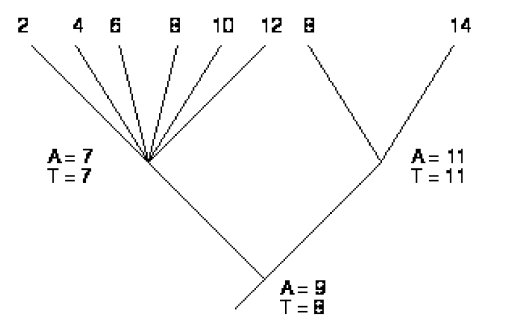
\includegraphics[width=10cm]{img/fig1.jpg}
\caption{Illustration of calculation of weighted trait averages ($A$) and tip averages ($T$) on a phylogeny}
\label{fig1}
\end{figure}


The mean and standard deviation of the tip values ($C$) may be more
appropriate for floristic and community studies, where the taxa in a
particular clade are a biogeographic or ecological subset from the
underlying phylogeny. The mean and variance of $A_{i,j}$ provide a more
direct measure of evolutionary divergence and are appropriate for
historical inference from data sets sampled from across entire
clades. A values are also less sensitive to differences in sampling
intensity across clades.

The significance of $A$, $D$, $T$, and $S$ at each node are all
assessed by randomization (see below). Significantly higher or low
values of $A$ and $T$ indicate that the clade in question has lower or
higher mean trait values that expected by chance. Significant results
for $D$ and $S$ indicate low or high levels of diversification at a node
($D$) or overall diversification within a clade ($S$)
\citep[see][]{losos2002tes, ackerly2004evo}.

\subsection{The Contribution Index: Node-based partitioning of trait
  variance}

\citet{moles2005briX} introduced new statistics to calculate the
contribution of each divergence in a phylogeny to the overall variance
in trait values across species. The following parameters are
calculated to generate the `Contribution Index' (see worked example in
supplementary material to \citet{moles2005briX}. The following
parameters are calculated and reported by {\scshape phylocom}, where the
final three parameters correspond to Steps 2, 3 and 4 outlined in the
\citet{moles2005briX} supplementary material.

\textit{NB: Previous users of AOT should note that the variables
  output by the program have been changed in v3.1 and onwards; output
  from previous versions did not exactly match the
  \citet{moles2005briX} paper.}

\begin{description}
\item[\hspace{1em} SSTipsVNode] total sum of squares for trait variance among
  species, relative to the nodal value for a clade (Ai). This is
  equivalent to the sums of squares of standard statistics, except
  deviations of each trait values are calculated relative to the nodal
  trait value at the base of each clade, rather than the grand
  mean. The result will necessarily be somewhat higher than the normal
  sums of squares.
\item[\hspace{1em} SSAmongNodes] sum of squares of the variance among nodal trait
  values of daughter nodes immediately subtending each node of the
  tree, weighted by the number of taxa in each node. This measures the
  among clade variance for the clades descendent from each node.
\item[\hspace{1em} SSWithinNodes] sum of squares of the variance among species
  trait values within each daughter clade descendent from a node. This
  is the sum of the individual SSTipsVNode values for those clades.
\item[\hspace{1em} PercVarAmongNodes] The percent of total trait variance in a
  clade that is explained by the divergence among daughter clades $=
  SSAmongNodes / (SSAmongNodes + SSWithinNodes)$.
\item[\hspace{1em} PercVarAtNode] The percent of total trait diversity that is
  contributed by the clade defined by this node $=
  SSTipsVNode / SSTipsVNode(root)$ 
\item[\hspace{1em} ContributionIndex] $PercVarAmongNodes \times PercVarAtNode$
\end{description}

\subsection{Phylogenetic independent contrasts}

AOT calculates evolutionary correlations between traits using
independent contrasts. This method and its assumptions has been
discussed extensively elsewhere and the user is advised to consult
\citet{felsenstein1985phy, garland1992pro} for a thorough
introduction. For pairs of continuous traits, AOT calculates
standardized independent contrasts based on the branch lengths in the
phylogeny (see below). Significance testing of the resulting
correlation values can be done using tables of critical values for the
Pearson correlation coefficient.

Independent contrasts are calculated from internal node averages ($A$
values) of daughter nodes at each node. The direction of subtraction
is set so that the sign of the contrast on trait 1 (X) is positive,
and traits 2 and above (Y) are then compared in the same direction
across the node. To handle polytomies, AOT uses the method introduced
by \citet{pagel1992met} to obtain a single degree of freedom contrast at each
polytomy, treating the polytomies as `soft'. In this method, one trait must be designated as the
independent or X variable, and all other traits are dependent or Y
variables. The nodes arising from a polytomy are then ranked based on
the values of trait X (see below for specifying which trait in a data
set is set as X). The species are then split into two groups. For
continuous traits, they are split at the median (if there are an odd
number, the median value is assigned to the lower group if its value
is lower than the mean for the entire set, and vice versa). For binary
traits, they are split into groups by state. Then the mean values for
all traits are calculated for the two groups, and the difference
between these means is taken as a single contrast. This maximizes the
difference in means for trait X, and the other traits fall out
according to their distribution between the two groups.

AOT tests independent contrasts between continuous traits, or between
continuous traits and a binary trait. Correlations between continuous
traits are calculated over $N-1$ internal traits. Contrasts on
discrete traits can only be calculated on a limited set of nodes,
where contrasting states of the binary trait occur on at least two of
the descendent nodes (\citealt{purvis2003com}; also see
\citealp{maddison2000tes}). AOT identifies two sets of nodes for
binary contrasts: the sister-taxa (ST) set and the paraphyletic (PT)
set (Fig.~\ref{fig2}). The ST contrasts involve nodes at which both
binary states are observed in the daughter nodes, and no daughter
clades contain a mix of the two states. Once a node is designated as
ST, no deeper nodes on the path from that node to the root can be
designated as an ST contrast.  Some of these deeper nodes can be
selected as PT contrasts, based on the rule that the paths connecting
taxa that form a contrast cannot cross. PT contrasts are designated by
pruning any node that has already been used as a contrast (ST or PT),
and then continuing up the tree looking for bifurcations between the
two binary states (Fig.~\ref{fig2}). AOT reports results for contrasts
calculated on the ST set alone, or on the combined ST+PT sets. I
believe that the CAIC BRUNCH algorithm \citep{purvis2003com} also uses
the combined ST+PT set of contrasts, but I have not confirmed this
yet.

\begin{figure}[!ht]
\centering
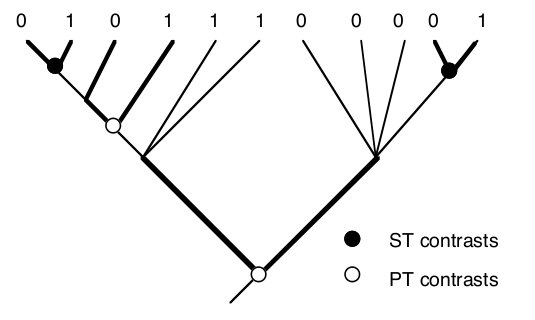
\includegraphics[width=10cm]{img/fig2.jpg}
\caption{Illustration of nodes selected for ST and PT contrasts on a binary trait.}
\label{fig2}
\end{figure}

For pairs of continuous characters, AOT outputs the correlation of
independent contrasts, the significance based on randomization, and
the sample size (= number of internal nodes). For a continuous vs. a
binary character, results are output for the ST and combined sets; for
each one, the output consists of a paired t-test (the average
magnitude of the continuous trait contrast for the available nodes and
its significance), and a sign test (the number of positive contrasts
for the continuous trait, the total number of contrasts, and the
significance of the sign test).

\subsection{Branch lengths}

The theory of independent contrasts relies heavily on the use of
appropriate branch lengths on the phylogeny, in units of `expected
character evolution' \citep{felsenstein1985phy}. However, it is very
difficult to justify the choice of BL distributions (e.g., based on
molecular data) for analysis of ecological and morphological
traits. Numerous simulation and empirical studies have shown that the
results of most independent contrasts analyses are quite robust to
different BL distributions \citep[e.g.,][]{diazuriarte1996tes,
  ackerly2000tax}. Several tests can be applied to test whether a
particular data set fits the expectation of Brownian motion, as
assumed by independent contrasts. One of these is to test for a lack
of correlation between the absolute value of standardized contrasts
and the underlying standardization term \citep[square root of the sum
  of the subtending branch lengths,][]{garland1992pro}. These terms
are output by {\scshape phylocom} (\verb|aotf| option) and can be
imported and tested in any statistics package. The \verb|Continuous|
program \citep{pagel1999inf} implements maximum likelihood tests of
several different parameters, representing deviations from Brownian
Motion; this program is also now implemented in \verb|BayesTraits|
\citep{pagel2006bay}.  \citet{oliver2007mod} discuss several other
testable assumptions derived from Brownian motion.

The \verb|-e| switch in {\scshape phylocom} will disable standardization of
contrasts, and output unstandardized contrasts and their
correlations. Note that this is not exactly the same as setting all
branch lengths = 1. Under Felsenstein's algorithm, deeper branches are
elongated during the calculation of contrasts, to reflect greater
uncertainty at deeper nodes. This step can be applied to equal branch
lengths, such that the deeper nodes will effectively have branch
lengths slightly greater than 1. To use equal branch lengths with
standardization in {\scshape phylocom}, branch lengths must be either
deleted or set to 1 in the tree file.  

\subsection{Significance testing}

Significance testing for all node-level and tree-wise conservatism
measures is conducted by randomization of trait values across the tips
of the phylogeny. Results of randomization are reported as the number
of randomizations for which the statistic was less than or equal to
the observed data (PL), and the number for which it was greater than
or equal to the observation (PH), including the observation (see
below). By default 999 randomizations are perfomed, plus the observed
data for a total of 1,000. The number of randomizations can be set
using the \verb|-r| switch, to obtain higher precision in significance
values; to obtain observed values only without significance testing,
use \verb|-r 0|.

Significance for one-tailed tests can be calculated as p = PL/R or p =
PH/R, if testing for observations that are lower than expected or
higher than expected, respectively. For two-tailed tests: p =
minimum(2PL/R, 2PH/R).

For large sample sizes, the calculation of PL and PH separately is
redundant, because PL+PH = R+1 (e.g., if the observation was lower
than all 999 random replicates, PL = 1 and PH = 1000). However, for
very small sample sizes, where randomization may result in many
identical outcomes, PL and PH may sum to more than R+1. This occurs
because all randomizations that result in values identical to the
observation should be counted in both PL and PH (since significance is
for randomizations less than or \textit{equal to} the observation). PL
and PH are both tabulated to address this situation.

\subsubsection{Significance of independent contrasts}

Randomization of tip values is not appropriate for testing independent
contrasts, because it breaks down patterns of trait conservatism
\citep[see][]{lapointe2001gen}. Significance of contrasts should be
determined from appropriate parametric tests. For pairs of continuous
traits, the correlation coefficient for independent contrasts can be
tested for significance, using N-1 df (where N is the number of
internal nodes providing contrasts) \citep[][Table
  R]{rohlf1995sta}. For tests of a continuous trait vs. a discrete
trait, the mean and standard deviation of of the contrasts can be used
to conduct a one-sample t-test against the null hypothesis that the
mean = 0. This is based on a t-statistic with N-1 df (where N is
number of contrasts again) \citep[see][Table B]{rohlf1995sta}, and is
equivalent to a paired t-test conducted across the contrast
nodes. (Note: currently {\scshape phylocom} only calculates
unstandardized contrasts if trait 1 is binary. To obtain standardized
contrasts, which may be more appropriate for the one-sample t-test
approach, the analysis could be run once with x 1 binary, to determine
which nodes are identified as `ST' and `PT', and then run again with x
1 set to continuous to obtain standardized contrasts for the remaining
traits.) Finally, significance of a sign test can be tested against
the binomial expectation \citep[][Table Q]{rohlf1995sta}.

\subsection{Phylogenetic signal}

Phylogenetic signal is measured using a test based on the variance of
standardized independent contrasts \citep{blomberg2002tem, blomberg2003tes}.
If related species are similar to each other, the magnitude of independent
contrasts will generally be similar across the tree, resulting in a
small variance of contrast values. Observed contrast variances are
compared to the expectations under a null model of randomly swapping
trait values across the tips of the tree.

Note that in previous versions of Phylocom ($<$4.0), phylogenetic
signal was calculated using a different method, based on the average
magnitude of unstandardized independent contrasts over the tree. The
current method will give different results than the previous method,
especially since it is based on standardized contrasts which take
branch length information into account. However, by taking branch lengths
into account, the method provides a useful complement to other model-based measures of
phylogenetic signal such as the \textit{K} statistic of \citet{blomberg2002tem}. Phylogenetic signal
calculations may result in NA values when the x variable is binary,
since contrasts are only calculated for nodes at which there is a
contrast in the binary trait. In this case, try setting the x variable
to be continuous with the \texttt{-x} switch (see section
\ref{aotswitch}).

\subsection{Running trait analyses}

Trait analyses can be run in three ways, each of which provides
different output formats:

\begin{itemize}
\item[] \texttt{aot} space-delimited output formatted for screen
\item[] \texttt{aotf} tab-delimited output for spreadsheet
\item[] \texttt{aotn} Nexus-formatted output for visualization in Mesquite
\end{itemize}

\subsubsection{Switches}
\label{aotswitch}

\begin{itemize} \raggedright
\item[] \texttt{-r INT} Modifies the number of randomizations (default
  = 999). E.g., \verb|$ phylocom aot -r 99|
\item[] \texttt{-x INT} Specify which trait should be used as x
  variable for contrasts (default = 1). E.g., \verb|$ phylocom aot -x 2|
\item[] \texttt{-e} Use equal branch lengths and unstandardized contrasts
\end{itemize}

To output results to a file, add a file name:
\begin{verbatim}
  $ phylocom aotf > results.txt
\end{verbatim}

Any number of switches can be combined in any order, e.g.:
\begin{verbatim}
  $ phylocom aot -r 99 -e -x 3 > results.txt
\end{verbatim}

\subsection{Output format}

The output has four different tables: individual node statistics;
independent contrast values; tree-wide phylogenetic signal;
correlations of independent contrasts. Option \verb|aot| provides
tables 3 and 4 only, formatted for viewing on the screen
(space-delimited). Option \verb|aotf| provides all four tables in a
table-delimited table best viewed in a spreadsheet program. On a Mac,
use the \verb|open| command to open this file directly from the command line:
\verb|open -a Microsoft\ Excel results.txt|. Option \verb|aotn| produces a
Nexus-format file for opening in Mesquite.

\subsubsection{Output table 1: Trait conservatism by node (\texttt{aotf} only)}

Column headings:

\begin{description}
\item[\hspace{1em} trait] trait number
\item[\hspace{1em} trait.name] trait name if provided in line 2 of the traits file;
  otherwise \verb|trait_#|
\item[\hspace{1em} node] node number
\item[\hspace{1em} name] node name (last column in screen formatted output)
\item[\hspace{1em} age] node age, based on branch lengths in phylo file
\item[\hspace{1em} N.tax] number of terminal taxa descended from node
\item[\hspace{1em} N.nodes] number of daughter nodes descended from node (= 2 for bifurcating nodes)
\item[\hspace{1em} Tip.mn] Mean value of trait across all descendent terminal taxa ($T$)
\item[\hspace{1em} Tmn.rankLow] Significance of mean, rank in low tail of null
  distribution (sig in screen output)
\item[\hspace{1em} Tmn.rankHi] Significance of mean, rank in high tail of null
  distribution
\item[\hspace{1em} Tip.sd] Standard deviation of trait values across all descendent terminal taxa (`tips')
\item[\hspace{1em} Tsd.rankLow] Significance of standard deviation, rank in low tail of null distribution
\item[\hspace{1em} Tsd.rankHi] Significance of standard deviation, rank in high tail of null distribution
\item[\hspace{1em} Node.mn] Mean trait value calculated under ancestral averaging algorithm (A)
\item[\hspace{1em} Nmn.rankLow] Significance of ancestral mean value, rank in low tail of null distribution
\item[\hspace{1em} Nmn.rankHi] Significance of ancestral mean value, rank in high tail of null distribution
\item[\hspace{1em} Nod.sd] Standard deviation of values at daughter nodes (`divergences'); measure of trait radiation at this node
\item[\hspace{1em} Nsd.rankLow] Significance of divergence deviation, rank in low tail of null distribution
\item[\hspace{1em} Nsd.rankHi] Significance of divergence deviation, rank in high tail of null distribution
\item[\hspace{1em} SSTipsRoot] Standard sum of squares of trait variance for all species
\item[\hspace{1em} SSTips] Standard sum of squares of trait variance for species descended from this node
\item[\hspace{1em} percVarAmongNodes] Percent of variance in clade contributed by divergence at this node
\item[\hspace{1em} percVarAtNode] Percent of all trait variance contributed by
  species at this node
\item[\hspace{1em} Contribution] Contribution of divergence at this node to overall
  species level variation in
\item[\hspace{1em} Index] trait \citep[see][]{moles2005briX}
\item[\hspace{1em} SSTipVNodeRoot] Sums of squares of trait deviations from nodal
  trait value at root
\item[\hspace{1em} SSTipVNode] Sums of squares of trait deviations from nodal trait value at this node
\item[\hspace{1em} SSAmongNodes] Sums of squares of deviations of daughter node trait
  values from nodal trait values at this node
\item[\hspace{1em} SSWithinNodes] Sums of squares of deviations of species trait
  values within subclades descended from this node
\end{description}


\subsubsection{Output table 2: Independent contrasts by node (\texttt{aotf} only)}

The LowVal and HiVal columns allow plotting of paired trait values in
the original trait space that are then used to calculate
contrasts. Column headings:

\begin{description}

\item[\hspace{1em} node] node number
\item[\hspace{1em} name] node name (last column in screen formatted output)
\item[\hspace{1em} age] node age, based on branch lengths in phylo file
\item[\hspace{1em} N.nodes] number of daughter nodes descended from
  node (= 2 for bifurcating nodes)
\item[\hspace{1em} Contrast1] Magnitude of independent contrasts for
  trait 1
\item[\hspace{1em} Contrast2] Magnitude of independent contrasts for trait 2
\item[\hspace{1em} ...] columns for any additional traits
\end{description}

\noindent If x is binary:

\begin{description}
\item[\hspace{1em} NodeType] PT: paraphyletic contrasts; ST: sister-taxon contrasts. See discussion of binary traits above.
\end{description}

\noindent If x is continuous:

\begin{description}
\item[\hspace{1em} ContrastSD] Standard deviation of the contrast (square root of sum of subtending branch lengths)
\item[\hspace{1em} LowVal1] Lower node value used for calculating contrast 1
\item[\hspace{1em} HiVal1] Higher node value used for calculating contrast 1
\item[\hspace{1em} LowVal2] Node value for trait 2 at node with lower value for trait 1
\item[\hspace{1em} HiVal2] Node value for trait 2 at node with higher value for trait 1
\item[\hspace{1em} ...] 	node values for additional traits
\end{description}

\subsubsection{Output table 3: Trait conservatism---treewise results}

Column headers:

\begin{description}

\item[\hspace{1em} Trait] Trait name (or number in screen output)
\item[\hspace{1em} NTaxa] Total number of taxa in tree
\item[\hspace{1em} VarCn] Variance of standardized contrasts across tree
\item[\hspace{1em} VarCn.rankLow] Significance of contrast variance relative to
  null model, low rank
\item[\hspace{1em} VarCn.rankHi*] Significance of contrast variance relative to
  null model, high rank
\end{description}

\subsubsection{Output table 4: Independent contrast correlations}

Results for traits 2 and higher vs. trait 1. If trait 1 is continuous,
column headers are as follows (*: `aotf' only):

\begin{description}
\item[\hspace{1em} Trait] Number for trait Y (`aot' only)
\item[\hspace{1em} XTrait*] Name for trait X (same for all rows)
\item[\hspace{1em} YTrait*] Name for trait Y
\item[\hspace{1em} NTaxa*] Total number of taxa
\item[\hspace{1em} PicR] Correlation of independent contrasts
\item[\hspace{1em} nPos] Number of positive contrasts for sign test
\item[\hspace{1em} nCont] Number of contrasts tested
\end{description}

\noindent If trait 1 is binary, then the columns are:

\begin{description}	
\item[\hspace{1em} Tr] Trait number (\verb|aot| only)
\item[\hspace{1em} XTrait*] Name for trait X (same for all rows)
\item[\hspace{1em} YTrait*] Name for trait Y
\item[\hspace{1em} NTaxa*] Total number of taxa
\item[\hspace{1em} MnConAll] Average magnitude of independent
  contrasts across all contrasts (subtracting node with lower value
  for binary character from node with higher value)
\item[\hspace{1em} SdConAll] Standard deviation of independent
  contrasts across all contrasts (for use in one-sample t-test)
\item[\hspace{1em} nPosAll] Number of positive contrasts for sign
  test, across all contrasts
\item[\hspace{1em} nContAll] Total number of contrasts tested (ST+PT)
\item[\hspace{1em} ] (Next 4 columns repeat 4 above, for ST contrasts only)
\end{description}


\section{Afterword}

Please feel free to read the code for details of what is done---it's
heavily commented. If you have any comments or questions (even trivial
ones), feel free to email us. If you think something is not working
right, PLEASE get in touch. We have tried to assure that the
algorithms are correct, but some errors are hard to spot.

There is much still to be added to {\scshape phylocom} (incorporating
tree conversions, link character value analyses to community
structure, etc.). If you have an algorithm you'd like implemented, let
us know.

\section{Citing {\scshape phylocom}}

If you use {\scshape phylocom}, please cite the software in any resulting publications:

\begin{raggedright}
\begin{itemize}
 \item[] Webb, C.\ O., Ackerly, D.\ D., and Kembel, S.\ W. 2008. Phylocom: software for the analysis of
phylogenetic community structure and character evolution. Bioinformatics 24: 2098-2100.
\end{itemize}
\end{raggedright}


\section{Acknowledgments}

\textit{Cam}: The original idea for these analyses came from the work
of researchers in the 60's and 70's on species/genus ratios. David
Baum suggested adding nearest-phylogenetic-neighbor metrics. Michael
Donoghue and David Ackerly have both influenced my software ideas
greatly.  Phylocom development has been supported by grants 0212873
and 0515520 from the US \htmladdnormallink{NSF}{http://www.nsf.gov/},
by \htmladdnormallink{The Arnold Arboretum of Harvard
  University}{http://www.arboretum.harvard.edu/}, and the
\htmladdnormallink{Yale Institute of Biospheric
  Studies}{http://www.yale.edu/yibs/}.


\bigskip \noindent \textit{David}: Thanks to Michael Donoghue for his
inspiration in the pursuit of `tree-thinking', to Mark Westoby and
Angela Moles for assistance with the `Contribution Index', and to Cam
for enthusiasm and support in development of AOT. The implementation
of the AOT module was facilitated by an NCEAS workshop on Neotropical
forest ecology, co-organized with Susan Mazer and Miguel
Martinez-Ramos.

\bigskip \noindent \textit{Steve}: Thanks to Mark Dale, whose collection of BASIC code
first inspired me to learn scientific programming. Thanks to NSERC for support.

\section{Legal}

This software is Free and Open Source, distributed under a BSD
(`3-clause') license:

{\scshape phylocom} Version \phylocomversion~\copyright~2009 Campbell
O.\ Webb, David D.\ Ackerly, Steven W.\ Kembel. All rights reserved.

Redistribution and use in source and binary forms, with or without
modification, are permitted provided that the following conditions are
met:
\begin{compactitem}

    \item Redistributions of source code must retain the above copyright
      notice, this list of conditions and the following disclaimer.
    \item Redistributions in binary form must reproduce the above
      copyright notice, this list of conditions and the following
      disclaimer in the documentation and/or other materials provided
      with the distribution.
    \item The names of the authors may not be used to endorse or promote
      products derived from this software without specific prior
      written permission.

\end{compactitem}

 THIS SOFTWARE IS PROVIDED BY THE COPYRIGHT HOLDERS AND CONTRIBUTORS
 ``AS IS'' AND ANY EXPRESS OR IMPLIED WARRANTIES, INCLUDING, BUT NOT
 LIMITED TO, THE IMPLIED WARRANTIES OF MERCHANTABILITY AND FITNESS FOR
 A PARTICULAR PURPOSE ARE DISCLAIMED. IN NO EVENT SHALL THE COPYRIGHT
 OWNER OR CONTRIBUTORS BE LIABLE FOR ANY DIRECT, INDIRECT, INCIDENTAL,
 SPECIAL, EXEMPLARY, OR CONSEQUENTIAL DAMAGES (INCLUDING, BUT NOT
 LIMITED TO, PROCUREMENT OF SUBSTITUTE GOODS OR SERVICES; LOSS OF USE,
 DATA, OR PROFITS; OR BUSINESS INTERRUPTION) HOWEVER CAUSED AND ON ANY
 THEORY OF LIABILITY, WHETHER IN CONTRACT, STRICT LIABILITY, OR TORT
 (INCLUDING NEGLIGENCE OR OTHERWISE) ARISING IN ANY WAY OUT OF THE USE
 OF THIS SOFTWARE, EVEN IF ADVISED OF THE POSSIBILITY OF SUCH DAMAGE.


\addtolength{\bibsep}{-8pt}
%\bibliographystyle{ecology_nourl}
\bibliographystyle{ecology}
\begin{raggedright}
\bibliography{phylocom_manual.bib} \addcontentsline{toc}{section}{References}
\end{raggedright}

\appendix

\section{Appendix: Worked examples}

Notation: \verb|#| begins a comment line. \verb|$| indicates a command
that can be run at a unix command prompt.

\subsection{Make a phylogeny for a plant species list}

\begin{verbatim}
# Copy a recent megatree from phylomatic (e.g. using curl)
$ curl http://svn.phylodiversity.net/tot/megatrees/R20080401.new > \
  R20080401.new

# Create a species list in the appropriate format, called taxa
$ cat taxa
Annonaceae/Annona/Annona_cherimola
Annonaceae/Annona/Annona_muricata
Fagaceae/Quercus/Quercus_robur
...

# Run phylomatic
$ ./phylomatic -f R20080401.new
$ ./phylomatic -f R20080401.new > myphylo
$ cat myphylo

\end{verbatim}

\section{Appendix: FAQs}

\setlength{\parindent}{0in}
\setlength{\parskip}{8pt}

\subsection{Running {\scshape phylocom}}

\textit{``I called my phylogeny file} \verb|phylo|, \textit{but}
       {\scshape phylocom} \textit{says it can't find the phylogeny
         file?''}  (Windows users) By default, Windows prevents users
       from seeing full filenames, hiding the (usually
       three-character) suffix.  This default behavior can be turned
       off in the `Folder options' of the Control Panel, which we
       recommend strongly for serious computer users.  If you created
       a \verb|phylo| file in an editor, there is good chance it is
       actually called \verb|phylo.txt|, which phylocom will not find.

\subsection{AOT}

\textit{``In the AOT module, I get output that contains `NaN' and/or
  `Inf'?''}  This is usually due to having resolved a polytomy as zero
length branches. Standardized contrasts are divided by the sum of
subtending branch lengths, and this will result in `Inf' if it divides
by zero. Another possible explanation is that the x variable (set with
the \texttt{-x} switch) is a binary trait. In this case, contrasts are only
calculated at nodes for which there is a contrast in the x variable,
which can lead to NaN values when there
are relatively few nodes with contrasts calculated.

\textit{``I still don't really understand the tree-wide statistic
  that AOT calculates.''}  AOT implements an algorithm that is
discussed by \citet{blomberg2003tes} in \textit{Evolution}. It is not
the $K$ statistic, but in the earlier part of the paper they talk about
using the variance of standardized contrasts as a measure of signal,
and comparing it to a null hypothesis of random shuffling of tip values
across the tree. Note that by this measure Brownian motion will
provide traits with a high degree of signal. This randomization
approach cannot tell you if your traits are more or less conserved
than expected under Brownian motion. For that you need a statistic
such as $K$ or another approach to randomization than we have
implemented.

\textit{``How does AOT compare to CAIC?''}  If you are analyzing
variation in a continuous trait Y relative to a discrete trait X, then
phylocom implements the \texttt{BRUNCH} algorithm of
\texttt{CAIC}. This will ignore the variance in Y observed across
contrasts where X is constant.

\subsection{BLADJ}

\textit{``How can I run {\sc bladj} on a set of randomly resolved
  trees?''}  Answer: with a bit of (unix) shell scripting.  E.g.
\begin{verbatim}
  #!/bin/sh
  # rndres2bl.sh 
  # Takes a randomly resolved set of trees as input, matches to a tree
  #   with interior node names, and then runs bladj.  Assumes that the
  #   comnode match codes (match0...n) always occur in the same place.
  # Input files: 
  #   1. infile.nex, a NEXUS file, with trees beginning, e.g.:
  #      TREE rnd_resol1 = [&R] (((A,B),C),((D,E),F));
  #   2. tree1, an unresolved tree to match against, e.g.:
  #      ((A,B,C)cladeA,(D,E,F)cladeD);
  #   3. ages, a bladj ages file, e.g.:
  #     match0    100
  #     match1    60
  #     match2    30
  # Creating the ages file will take a bit of visual assessment to
  #   work out which of the matchX nodes can be dated.

  grep "^TREE\ rnd" infile.nex | sed \
    's/^TREE\ *rnd_resol[0-9]*\ *=\ *\[\&R\]\ *//g' > infile2.nex
  N=0
  echo -e "#NEXUS\nBEGIN TREES;" > outfile.nex
  for tree in `grep ";" infile2.nex`
  do
    echo $tree > tree2
    phylocom comnode > matched.nex
    grep "^TREE\ tree2" matched.nex | \
      sed 's/TREE\ tree2\ =\ //g' > phylo
    let N=$N+1
    echo -n "TREE rnd_resol"$N" = [&R] " >> outfile.nex
    phylocom bladj >> outfile.nex
  done
  echo "END;" >> outfile.nex
  rm -f infile2.nex tree2 matched.nex
\end{verbatim}

\subsection{new2nex and makenex}

\textit{``I get this error when importing a .nex file into Mesquite:
Taxon name in translation table doesn't correspond to name of
known taxon ("," [a])''}  This appears to be an issue with some
new versions of Mesquite, and might be fixed with postprocessing the
nexfile using this command (thanks to Adam Wolf):
\begin{verbatim}
  $ sed '/TRANSLATE/,/TREE/ s/, /   /g' infile.nex > outfile.nex
\end{verbatim}


\subsection{Phylomatic}

\textit{``Why won't the megatrees (e.g., R20081027.new) open in
  TreeViewX?''} The phylomatic database allows single daughter nodes
in Newick: ((A,B)C)D which are also allowed by the Newick standard.
\htmladdnormallink{TreeViewX}{http://darwin.zoology.gla.ac.uk/~rpage/treeviewx/}
can also handle these, but seems not to like it when the files are
large.  The single daughter nodes can be cleaned out using phylocom,
e.g.:
\begin{verbatim}
  $ phylocom cleanphy -e -f R20081027.new > clean.new
\end{verbatim}
The resulting file will open in TreeViewX.  I have found that
\htmladdnormallink{ATV}{http://www.phylosoft.org/atv/} can open the
files directly.  

Some other programs may also have trouble reading single daughter
nodes, or the \texttt{:0.0000} branch length of the root node, or even
any root node branch length at all, although these are all allowed by
the semi-formal \htmladdnormallink{Newick
  standard}{http://evolution.genetics.washington.edu/phylip/newick_doc.html}. If
you have trouble reading a phylocom or phylomatic tree into another
program, please open the file in a text editor and consider the above
issues.

{\bf PLEAE NOTE}: Issues of compatability fo the root
\verb|(...)euphyllophyte;| node and other software applications are
very common.  If you are having trouble, please remove this node
(edit out the \verb|(| and the \verb|)euphyllophyte;|) first. This can
be automated with:

\begin{footnotesize}
\begin{verbatim}
  sed -e 's/(//1' -e 's/)euphyllophyte:1.000000//1' -e 's/)euphyllophyte//1'
\end{verbatim}
\end{footnotesize}
\end{document}
